\documentclass[]{article}
\usepackage[T1]{fontenc}
\usepackage{lmodern}
\usepackage{amssymb,amsmath}
\usepackage{ifxetex,ifluatex}
\usepackage{fixltx2e} % provides \textsubscript
% use upquote if available, for straight quotes in verbatim environments
\IfFileExists{upquote.sty}{\usepackage{upquote}}{}
\ifnum 0\ifxetex 1\fi\ifluatex 1\fi=0 % if pdftex
  \usepackage[utf8]{inputenc}
\else % if luatex or xelatex
  \ifxetex
    \usepackage{mathspec}
    \usepackage{xltxtra,xunicode}
  \else
    \usepackage{fontspec}
  \fi
  \defaultfontfeatures{Mapping=tex-text,Scale=MatchLowercase}
  \newcommand{\euro}{€}
\fi
% use microtype if available
\IfFileExists{microtype.sty}{\usepackage{microtype}}{}
\usepackage[margin=1in]{geometry}
\usepackage{longtable,booktabs}
\usepackage{graphicx}
% Redefine \includegraphics so that, unless explicit options are
% given, the image width will not exceed the width of the page.
% Images get their normal width if they fit onto the page, but
% are scaled down if they would overflow the margins.
\makeatletter
\def\ScaleIfNeeded{%
  \ifdim\Gin@nat@width>\linewidth
    \linewidth
  \else
    \Gin@nat@width
  \fi
}
\makeatother
\let\Oldincludegraphics\includegraphics
{%
 \catcode`\@=11\relax%
 \gdef\includegraphics{\@ifnextchar[{\Oldincludegraphics}{\Oldincludegraphics[width=\ScaleIfNeeded]}}%
}%
\ifxetex
  \usepackage[setpagesize=false, % page size defined by xetex
              unicode=false, % unicode breaks when used with xetex
              xetex]{hyperref}
\else
  \usepackage[unicode=true]{hyperref}
\fi
\hypersetup{breaklinks=true,
            bookmarks=true,
            pdfauthor={Andresa de Andrade},
            pdftitle={Linear Regression},
            colorlinks=true,
            citecolor=blue,
            urlcolor=blue,
            linkcolor=magenta,
            pdfborder={0 0 0}}
\urlstyle{same}  % don't use monospace font for urls
\setlength{\parindent}{0pt}
\setlength{\parskip}{6pt plus 2pt minus 1pt}
\setlength{\emergencystretch}{3em}  % prevent overfull lines
\setcounter{secnumdepth}{5}

\title{Linear Regression}
\author{Andresa de Andrade}
\date{August 15, 2014}

\begin{document}

\begin{center}
\huge Linear Regression \\[0.2cm]
\end{center}
\begin{center}
\large \emph{Andresa de Andrade}\\[0.1cm]
\end{center}
\begin{center}
\large \emph{August 15, 2014} \\
\end{center}
\normalsize


{
\hypersetup{linkcolor=black}
\setcounter{tocdepth}{2}
\tableofcontents
}
\newpage 

\section{Summary of the data}\label{summary-of-the-data}

We'll be working with 60 observations of 10 guinea pigs. In this project
we are interested to know if there's difference in length of the teeth
for different levels of vitamin C and 2 deliver methods: orange juice
and ascorbic acid.

\section{Exploratory Analysis}\label{exploratory-analysis}

We need to check the 6 combinations of data (by supplement and by dose)

\begin{verbatim}
## Warning: package 'pander' was built under R version 3.1.2
\end{verbatim}

\begin{longtable}[c]{@{}cccccc@{}}
\toprule\addlinespace
\begin{minipage}[b]{0.23\columnwidth}\centering
~
\end{minipage} & \begin{minipage}[b]{0.05\columnwidth}\centering
N
\end{minipage} & \begin{minipage}[b]{0.08\columnwidth}\centering
Mean
\end{minipage} & \begin{minipage}[b]{0.12\columnwidth}\centering
St.~Dev
\end{minipage} & \begin{minipage}[b]{0.07\columnwidth}\centering
Min
\end{minipage} & \begin{minipage}[b]{0.07\columnwidth}\centering
Max
\end{minipage}
\\\addlinespace
\midrule\endhead
\begin{minipage}[t]{0.23\columnwidth}\centering
\textbf{ToothGrowth}
\end{minipage} & \begin{minipage}[t]{0.05\columnwidth}\centering
60
\end{minipage} & \begin{minipage}[t]{0.08\columnwidth}\centering
18.81
\end{minipage} & \begin{minipage}[t]{0.12\columnwidth}\centering
7.64
\end{minipage} & \begin{minipage}[t]{0.07\columnwidth}\centering
4.2
\end{minipage} & \begin{minipage}[t]{0.07\columnwidth}\centering
33.9
\end{minipage}
\\\addlinespace
\begin{minipage}[t]{0.23\columnwidth}\centering
\textbf{Orange Juice}
\end{minipage} & \begin{minipage}[t]{0.05\columnwidth}\centering
30
\end{minipage} & \begin{minipage}[t]{0.08\columnwidth}\centering
16.96
\end{minipage} & \begin{minipage}[t]{0.12\columnwidth}\centering
8.26
\end{minipage} & \begin{minipage}[t]{0.07\columnwidth}\centering
4.2
\end{minipage} & \begin{minipage}[t]{0.07\columnwidth}\centering
33.9
\end{minipage}
\\\addlinespace
\begin{minipage}[t]{0.23\columnwidth}\centering
\textbf{Ascorbic Acid}
\end{minipage} & \begin{minipage}[t]{0.05\columnwidth}\centering
30
\end{minipage} & \begin{minipage}[t]{0.08\columnwidth}\centering
20.66
\end{minipage} & \begin{minipage}[t]{0.12\columnwidth}\centering
6.6
\end{minipage} & \begin{minipage}[t]{0.07\columnwidth}\centering
8.19
\end{minipage} & \begin{minipage}[t]{0.07\columnwidth}\centering
30.9
\end{minipage}
\\\addlinespace
\begin{minipage}[t]{0.23\columnwidth}\centering
\textbf{Dose = 0.5}
\end{minipage} & \begin{minipage}[t]{0.05\columnwidth}\centering
20
\end{minipage} & \begin{minipage}[t]{0.08\columnwidth}\centering
10.6
\end{minipage} & \begin{minipage}[t]{0.12\columnwidth}\centering
4.49
\end{minipage} & \begin{minipage}[t]{0.07\columnwidth}\centering
4.2
\end{minipage} & \begin{minipage}[t]{0.07\columnwidth}\centering
21.5
\end{minipage}
\\\addlinespace
\begin{minipage}[t]{0.23\columnwidth}\centering
\textbf{Dose = 1}
\end{minipage} & \begin{minipage}[t]{0.05\columnwidth}\centering
20
\end{minipage} & \begin{minipage}[t]{0.08\columnwidth}\centering
19.73
\end{minipage} & \begin{minipage}[t]{0.12\columnwidth}\centering
4.41
\end{minipage} & \begin{minipage}[t]{0.07\columnwidth}\centering
13.6
\end{minipage} & \begin{minipage}[t]{0.07\columnwidth}\centering
27.3
\end{minipage}
\\\addlinespace
\begin{minipage}[t]{0.23\columnwidth}\centering
\textbf{Dose = 2}
\end{minipage} & \begin{minipage}[t]{0.05\columnwidth}\centering
20
\end{minipage} & \begin{minipage}[t]{0.08\columnwidth}\centering
26.1
\end{minipage} & \begin{minipage}[t]{0.12\columnwidth}\centering
3.77
\end{minipage} & \begin{minipage}[t]{0.07\columnwidth}\centering
18.5
\end{minipage} & \begin{minipage}[t]{0.07\columnwidth}\centering
33.9
\end{minipage}
\\\addlinespace
\begin{minipage}[t]{0.23\columnwidth}\centering
\textbf{VC Dose = 0.5}
\end{minipage} & \begin{minipage}[t]{0.05\columnwidth}\centering
10
\end{minipage} & \begin{minipage}[t]{0.08\columnwidth}\centering
7.98
\end{minipage} & \begin{minipage}[t]{0.12\columnwidth}\centering
2.74
\end{minipage} & \begin{minipage}[t]{0.07\columnwidth}\centering
4.2
\end{minipage} & \begin{minipage}[t]{0.07\columnwidth}\centering
11.5
\end{minipage}
\\\addlinespace
\begin{minipage}[t]{0.23\columnwidth}\centering
\textbf{VC Dose = 1}
\end{minipage} & \begin{minipage}[t]{0.05\columnwidth}\centering
10
\end{minipage} & \begin{minipage}[t]{0.08\columnwidth}\centering
16.77
\end{minipage} & \begin{minipage}[t]{0.12\columnwidth}\centering
2.51
\end{minipage} & \begin{minipage}[t]{0.07\columnwidth}\centering
13.6
\end{minipage} & \begin{minipage}[t]{0.07\columnwidth}\centering
22.5
\end{minipage}
\\\addlinespace
\begin{minipage}[t]{0.23\columnwidth}\centering
\textbf{VC Dose =2}
\end{minipage} & \begin{minipage}[t]{0.05\columnwidth}\centering
10
\end{minipage} & \begin{minipage}[t]{0.08\columnwidth}\centering
26.14
\end{minipage} & \begin{minipage}[t]{0.12\columnwidth}\centering
4.79
\end{minipage} & \begin{minipage}[t]{0.07\columnwidth}\centering
18.5
\end{minipage} & \begin{minipage}[t]{0.07\columnwidth}\centering
33.9
\end{minipage}
\\\addlinespace
\begin{minipage}[t]{0.23\columnwidth}\centering
\textbf{OJ Dose = 0.5}
\end{minipage} & \begin{minipage}[t]{0.05\columnwidth}\centering
10
\end{minipage} & \begin{minipage}[t]{0.08\columnwidth}\centering
7.98
\end{minipage} & \begin{minipage}[t]{0.12\columnwidth}\centering
2.74
\end{minipage} & \begin{minipage}[t]{0.07\columnwidth}\centering
4.2
\end{minipage} & \begin{minipage}[t]{0.07\columnwidth}\centering
11.5
\end{minipage}
\\\addlinespace
\begin{minipage}[t]{0.23\columnwidth}\centering
\textbf{OJ Dose = 1}
\end{minipage} & \begin{minipage}[t]{0.05\columnwidth}\centering
10
\end{minipage} & \begin{minipage}[t]{0.08\columnwidth}\centering
16.77
\end{minipage} & \begin{minipage}[t]{0.12\columnwidth}\centering
2.51
\end{minipage} & \begin{minipage}[t]{0.07\columnwidth}\centering
13.6
\end{minipage} & \begin{minipage}[t]{0.07\columnwidth}\centering
22.5
\end{minipage}
\\\addlinespace
\begin{minipage}[t]{0.23\columnwidth}\centering
\textbf{OJ Dose =2}
\end{minipage} & \begin{minipage}[t]{0.05\columnwidth}\centering
10
\end{minipage} & \begin{minipage}[t]{0.08\columnwidth}\centering
26.14
\end{minipage} & \begin{minipage}[t]{0.12\columnwidth}\centering
4.79
\end{minipage} & \begin{minipage}[t]{0.07\columnwidth}\centering
18.5
\end{minipage} & \begin{minipage}[t]{0.07\columnwidth}\centering
33.9
\end{minipage}
\\\addlinespace
\bottomrule
\end{longtable}

Please consider Ascorbic Acid as VC and Orange Juice as OJ

\begin{table}[!htbp] \centering 
  \caption{Summary Table} 
  \label{} 
\begin{tabular}{@{\extracolsep{5pt}}lccccc} 
\\[-1.8ex]\hline 
\hline \\[-1.8ex] 
Statistic & \multicolumn{1}{c}{N} & \multicolumn{1}{c}{Mean} & \multicolumn{1}{c}{St. Dev.} & \multicolumn{1}{c}{Min} & \multicolumn{1}{c}{Max} \\ 
\hline \\[-1.8ex] 
Toothlength & 60   & 18.813 & 7.649 & 4.200 & 33.900 \\ 
\hline \\[-1.8ex]
Orange Juice & 30  & 20.660 & 6.605 & 8.200 & 30.900 \\
\hline \\[-1.8ex]
Ascorbic Acid & 30 & 16.960 & 8.266 & 4.200 & 33.900 \\ \\
\hline \\[-1.8ex]
dose = 0.5    & 20 & 10.605 & 4.499 & 4.200 & 21.500\\
\hline \\[-1.8ex]
dose = 1      & 20 & 19.730 & 4.415 & 13.60 & 27.300\\
\hline \\[-1.8ex]
dose = 2      & 20 & 26.100 & 3.774 & 18.50 & 33.900\\  \\
\hline \\[-1.8ex]
VC-dose = 0.5 & 10 & 07.980 & 2.746 & 4.200 & 11.500 \\
\hline \\[-1.8ex]
VC-dose = 1   & 10 & 16.770 & 2.515 & 13.60 & 22.500 \\
\hline \\[-1.8ex]
VC-dose = 2   & 10 & 26.140 & 4.797 & 18.50 & 33.900 \\ \\
\hline \\[-1.8ex]
OJ-dose = 0.5 & 10 & 13.230 & 4.459 & 8.200 & 21.500 \\
\hline \\[-1.8ex]
OJ-dose = 1   & 10 & 22.700 & 3.911 & 14.50 & 27.300 \\
\hline \\[-1.8ex]
OJ-dose = 2   & 10 & 26.060 & 2.655 & 22.40 & 30.900 \\
\hline \\[-1.8ex]
\end{tabular} 
\end{table}

\begin{itemize}
\item
  From the table above and the Figure 2 we can infer that the average of
  teeth length between guinea pigs that were fed with orange juice is
  slightly higher than the ones fed with ascorbic acid, also the
  variability is lower for orange juice. But we can't really say that
  there's a significant difference.
\item
  When we look at different doses of vitamin C we have a a increase of
  teeth length as the doses are higher and a decrease in variance as the
  doses get bigger.
\item
  And when check the combination between type of supplement and vitamin
  C doses, we have, again, a better performance of Orange Juice. For the
  first dose orange juice means is 60\% higher than VC and Sd is 60\%
  lower than VC (the lower the sd the better). Even though for dose =2
  we have a higher average for VC, the variance is almost twice as for
  the orange juice, what suggests outliers or the data is more disperse
  around the mean as we can see in the boxplot.
\item
  Normality Assumption : from the Figure 1, we can't really infer that
  we have a normal distribution because the presence of outliers is very
  strong in this model. Thus for tests purposes, we'll be using the
  T-student distribution.
\end{itemize}

\section{Statistics Tests}\label{statistics-tests}

Now that we have an idea of how data is distributed, lets check if we
can confirm with a statistic test. This is the test that we'll be
applying:

\def\oj{\rule{0pt}{1.0ex}orangejuice}
\def\vc{\rule{0pt}{1.0ex}ascorbicacid} $H_{0}: \mu_{\oj} = \mu_{\vc}$
versus $H_{1}: \mu_{\oj} \neq \mu_{\vc}$

Note: we don't have a paired test because we have different guinea pigs
tooth.

The p-value for difference in types of supplement(vc and oj) is greater
than 0.05, which suggests that there's no difference between orange
juice and ascorbic acid.

Let's test if there's difference between the doses of vitamin C:

According to the Figure 5, there's difference between treatment at 0.5
mg and 1mg. And the CI for 95\% of confidence is {[}-11.984, -6.276{]}.
So if the difference between means was within this interval (considering
absolute numbers), we could have inferred that there's no difference
between treatments.

According to the Figure 6, we also have the difference between
treatments from doses at 0.5 and at 1 not significant (p-value
\textless{}0.01).

Now to check if there's difference between treatment at dose = 1 and at
dose = 2 we go to Figure 7 and observe that the p-value is also very
low, so we can reject the null hypothesis of no difference between the
the treatments.

\newpage

\section{\#Appendix}\label{appendix}

Figure 1

\begin{figure}[htbp]
\centering
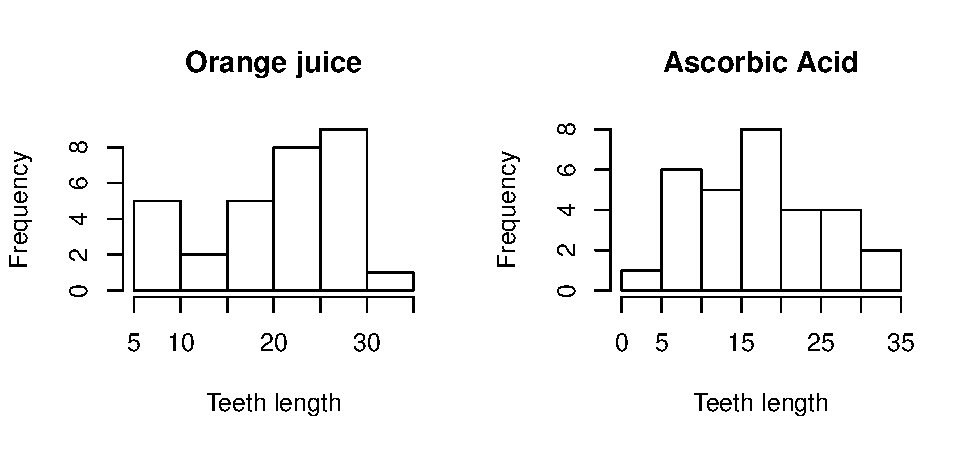
\includegraphics{./inference_project_part2_files/figure-latex/unnamed-chunk-3-1.pdf}
\end{figure}

\begin{figure}[htbp]
\centering
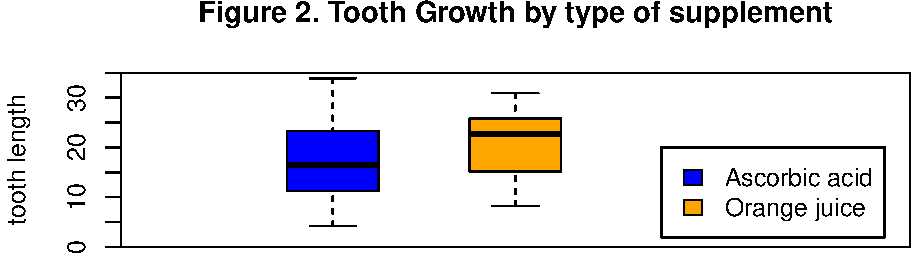
\includegraphics{./inference_project_part2_files/figure-latex/unnamed-chunk-4-1.pdf}
\end{figure}

Figure 4

\begin{verbatim}
## 
##  Welch Two Sample t-test
## 
## data:  vc_subset$len and oj_subset$len
## t = -1.9153, df = 55.309, p-value = 0.06063
## alternative hypothesis: true difference in means is not equal to 0
## 95 percent confidence interval:
##  -7.5710156  0.1710156
## sample estimates:
## mean of x mean of y 
##  16.96333  20.66333
\end{verbatim}

Figure 5 - Dose: 0.5 x 1

\begin{verbatim}
## [1] 16.5 16.5 15.2 17.3 22.5 17.3
\end{verbatim}

\begin{verbatim}
## 
##  Welch Two Sample t-test
## 
## data:  dose_05$len and dose_1$len
## t = -6.4766, df = 37.986, p-value = 1.268e-07
## alternative hypothesis: true difference in means is not equal to 0
## 95 percent confidence interval:
##  -11.983781  -6.276219
## sample estimates:
## mean of x mean of y 
##    10.605    19.735
\end{verbatim}

Figure 6 - Dose: 0.5 x 2

Figure 7 - Dose: 1 x 2

\begin{verbatim}
## 
##  Welch Two Sample t-test
## 
## data:  dose_2$len and dose_1$len
## t = 4.9005, df = 37.101, p-value = 1.906e-05
## alternative hypothesis: true difference in means is not equal to 0
## 95 percent confidence interval:
##  3.733519 8.996481
## sample estimates:
## mean of x mean of y 
##    26.100    19.735
\end{verbatim}

Figure 8 - Dose: 0.5 Orange Juice x Ascorbic Acid

\begin{verbatim}
## 
##  Welch Two Sample t-test
## 
## data:  vc_05$len and oj_05$len
## t = -3.1697, df = 14.969, p-value = 0.006359
## alternative hypothesis: true difference in means is not equal to 0
## 95 percent confidence interval:
##  -8.780943 -1.719057
## sample estimates:
## mean of x mean of y 
##      7.98     13.23
\end{verbatim}

Figure 9 - Dose: 1 Orange Juice x Ascorbic Acid

\begin{verbatim}
## 
##  Welch Two Sample t-test
## 
## data:  vc_1$len and oj_1$len
## t = -4.0328, df = 15.358, p-value = 0.001038
## alternative hypothesis: true difference in means is not equal to 0
## 95 percent confidence interval:
##  -9.057852 -2.802148
## sample estimates:
## mean of x mean of y 
##     16.77     22.70
\end{verbatim}

Figure 10 - Dose: 2 Orange Juice x Ascorbic Acid

\begin{verbatim}
## 
##  Welch Two Sample t-test
## 
## data:  vc_2$len and oj_2$len
## t = 0.0461, df = 14.04, p-value = 0.9639
## alternative hypothesis: true difference in means is not equal to 0
## 95 percent confidence interval:
##  -3.63807  3.79807
## sample estimates:
## mean of x mean of y 
##     26.14     26.06
\end{verbatim}

\end{document}
